% GNUPLOT: LaTeX picture with Postscript
\begingroup
  \makeatletter
  \providecommand\color[2][]{%
    \GenericError{(gnuplot) \space\space\space\@spaces}{%
      Package color not loaded in conjunction with
      terminal option `colourtext'%
    }{See the gnuplot documentation for explanation.%
    }{Either use 'blacktext' in gnuplot or load the package
      color.sty in LaTeX.}%
    \renewcommand\color[2][]{}%
  }%
  \providecommand\includegraphics[2][]{%
    \GenericError{(gnuplot) \space\space\space\@spaces}{%
      Package graphicx or graphics not loaded%
    }{See the gnuplot documentation for explanation.%
    }{The gnuplot epslatex terminal needs graphicx.sty or graphics.sty.}%
    \renewcommand\includegraphics[2][]{}%
  }%
  \providecommand\rotatebox[2]{#2}%
  \@ifundefined{ifGPcolor}{%
    \newif\ifGPcolor
    \GPcolortrue
  }{}%
  \@ifundefined{ifGPblacktext}{%
    \newif\ifGPblacktext
    \GPblacktextfalse
  }{}%
  % define a \g@addto@macro without @ in the name:
  \let\gplgaddtomacro\g@addto@macro
  % define empty templates for all commands taking text:
  \gdef\gplbacktext{}%
  \gdef\gplfronttext{}%
  \makeatother
  \ifGPblacktext
    % no textcolor at all
    \def\colorrgb#1{}%
    \def\colorgray#1{}%
  \else
    % gray or color?
    \ifGPcolor
      \def\colorrgb#1{\color[rgb]{#1}}%
      \def\colorgray#1{\color[gray]{#1}}%
      \expandafter\def\csname LTw\endcsname{\color{white}}%
      \expandafter\def\csname LTb\endcsname{\color{black}}%
      \expandafter\def\csname LTa\endcsname{\color{black}}%
      \expandafter\def\csname LT0\endcsname{\color[rgb]{1,0,0}}%
      \expandafter\def\csname LT1\endcsname{\color[rgb]{0,1,0}}%
      \expandafter\def\csname LT2\endcsname{\color[rgb]{0,0,1}}%
      \expandafter\def\csname LT3\endcsname{\color[rgb]{1,0,1}}%
      \expandafter\def\csname LT4\endcsname{\color[rgb]{0,1,1}}%
      \expandafter\def\csname LT5\endcsname{\color[rgb]{1,1,0}}%
      \expandafter\def\csname LT6\endcsname{\color[rgb]{0,0,0}}%
      \expandafter\def\csname LT7\endcsname{\color[rgb]{1,0.3,0}}%
      \expandafter\def\csname LT8\endcsname{\color[rgb]{0.5,0.5,0.5}}%
    \else
      % gray
      \def\colorrgb#1{\color{black}}%
      \def\colorgray#1{\color[gray]{#1}}%
      \expandafter\def\csname LTw\endcsname{\color{white}}%
      \expandafter\def\csname LTb\endcsname{\color{black}}%
      \expandafter\def\csname LTa\endcsname{\color{black}}%
      \expandafter\def\csname LT0\endcsname{\color{black}}%
      \expandafter\def\csname LT1\endcsname{\color{black}}%
      \expandafter\def\csname LT2\endcsname{\color{black}}%
      \expandafter\def\csname LT3\endcsname{\color{black}}%
      \expandafter\def\csname LT4\endcsname{\color{black}}%
      \expandafter\def\csname LT5\endcsname{\color{black}}%
      \expandafter\def\csname LT6\endcsname{\color{black}}%
      \expandafter\def\csname LT7\endcsname{\color{black}}%
      \expandafter\def\csname LT8\endcsname{\color{black}}%
    \fi
  \fi
  \setlength{\unitlength}{0.0500bp}%
  \begin{picture}(6236.00,3968.00)%
    \gplgaddtomacro\gplbacktext{%
      \colorrgb{0.50,0.50,0.50}%
      \put(547,819){\makebox(0,0)[r]{\strut{}\footnotesize -2}}%
      \colorrgb{0.50,0.50,0.50}%
      \put(547,1138){\makebox(0,0)[r]{\strut{}\footnotesize 0}}%
      \colorrgb{0.50,0.50,0.50}%
      \put(547,1456){\makebox(0,0)[r]{\strut{}\footnotesize $\pm$2}}%
      \colorrgb{0.50,0.50,0.50}%
      \put(547,1775){\makebox(0,0)[r]{\strut{}\footnotesize 0}}%
      \colorrgb{0.50,0.50,0.50}%
      \put(547,2094){\makebox(0,0)[r]{\strut{}\footnotesize $\pm$2}}%
      \colorrgb{0.50,0.50,0.50}%
      \put(547,2412){\makebox(0,0)[r]{\strut{}\footnotesize 0}}%
      \colorrgb{0.50,0.50,0.50}%
      \put(547,2731){\makebox(0,0)[r]{\strut{}\footnotesize $\pm$2}}%
      \colorrgb{0.50,0.50,0.50}%
      \put(547,3049){\makebox(0,0)[r]{\strut{}\footnotesize 0}}%
      \colorrgb{0.50,0.50,0.50}%
      \put(547,3368){\makebox(0,0)[r]{\strut{}\footnotesize 2}}%
      \colorrgb{0.50,0.50,0.50}%
      \put(660,503){\makebox(0,0){\strut{}\footnotesize $0$}}%
      \colorrgb{0.50,0.50,0.50}%
      \put(1457,503){\makebox(0,0){\strut{}\footnotesize $15$}}%
      \colorrgb{0.50,0.50,0.50}%
      \put(2254,503){\makebox(0,0){\strut{}\footnotesize $30$}}%
      \colorrgb{0.50,0.50,0.50}%
      \put(3052,503){\makebox(0,0){\strut{}\footnotesize $45$}}%
      \colorrgb{0.50,0.50,0.50}%
      \put(3849,503){\makebox(0,0){\strut{}\footnotesize $60$}}%
      \colorrgb{0.50,0.50,0.50}%
      \put(4646,503){\makebox(0,0){\strut{}\footnotesize $75$}}%
      \colorrgb{0.50,0.50,0.50}%
      \put(5443,503){\makebox(0,0){\strut{}\footnotesize $90$}}%
      \colorrgb{0.50,0.50,0.50}%
      \put(5556,1138){\makebox(0,0)[l]{\strut{}200}}%
      \colorrgb{0.50,0.50,0.50}%
      \put(5556,1775){\makebox(0,0)[l]{\strut{}300}}%
      \colorrgb{0.50,0.50,0.50}%
      \put(5556,2412){\makebox(0,0)[l]{\strut{}500}}%
      \colorrgb{0.50,0.50,0.50}%
      \put(5556,3049){\makebox(0,0)[l]{\strut{}750}}%
      \csname LTb\endcsname%
      \put(173,2093){\rotatebox{-270}{\makebox(0,0){\strut{}magnitude deviation / dB}}}%
      \put(5995,2093){\rotatebox{-270}{\makebox(0,0){\strut{}Frequency / Hz}}}%
      \put(3051,283){\makebox(0,0){\strut{}source azimuth $\sfsphphi[subscript=s]$ / deg}}%
    }%
    \gplgaddtomacro\gplfronttext{%
      \csname LTb\endcsname%
      \put(1716,3637){\makebox(0,0)[r]{\strut{}Ground\,Truth}}%
      \csname LTb\endcsname%
      \put(3363,3637){\makebox(0,0)[r]{\strut{}2.5D\,WFS}}%
      \csname LTb\endcsname%
      \put(5010,3637){\makebox(0,0)[r]{\strut{}2.5D\,ESA}}%
    }%
    \gplbacktext
    \put(0,0){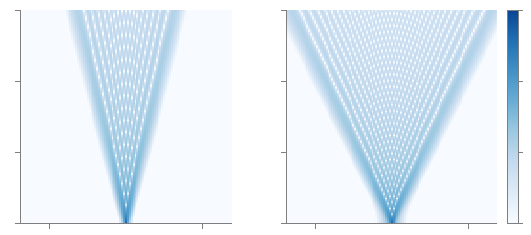
\includegraphics{fig}}%
    \gplfronttext
  \end{picture}%
\endgroup
